%!TEX root = root.tex

\chapter{HotMAPS: Exome-scale discovery of mutation hotspots in 3D protein structure}
\label{chap:ch5}
\chaptermark{HotMAPS}

\section{Introduction}

Missense mutations are perhaps the most difficult mutation type to interpret in human cancers. Truncating (loss-of-function) mutations and structural rearrangements generate major changes in the protein product of a gene, but a single missense mutation yields only a small change in protein chemistry. The impact of a missense mutation on protein function, cellular behavior, cancer etiology, and progression may be negligible or profound, for reasons that are not yet well understood. 

The recurrent observation across multiple cancer samples of missense mutations at the same amino acid residue position is well known to be a characteristic feature of both oncogenes (OG) and tumor suppressor genes (TSG; \cite{RN107}). The idea that somatic mutations also frequently occur in positions proximal in protein sequence to the most highly recurrent positions has suggested that positional clustering of somatic missense mutations might be used to identify drivers \cite{RN109}. These clusters, known as \q{hotspots,} are regions where somatic missense mutations occur closer together in protein sequence than would be expected by chance. Hotspot regions can be rationalized as areas in a protein under positive selection in the cancer environment; missense mutations occurring in these regions are selected for because they alter protein function in a manner advantageous to the cancer cell. Numerous methods have been developed to identify hotspots based on the linear protein sequence \cite{RN16, RN46, RN110, RN87, RN54, RN55}.

However, only using the linear sequence of a protein may fail to capture hotspots that appear in the 3-dimensional (3D) structure of a protein \cite{RN105}. Protein structure has long been known to relate to the function of a protein \cite{RN112, RN113}, and clustering of mutations within a structure may indicate mutations that are cancer drivers. A few algorithms leveraging this protein structure-function relationship have shown early signs of promise. An algorithm that leverages 3D protein structure information, but still performs clustering in 1D through a dimensionality reduction step, has shown utility in detecting oncogenes \cite{RN15}. A recent study of an aggregated collection of TCGA cancer mutations from 21 tumor types presented an algorithm to identify cancer genes based on 3D clustering of somatic missense mutations, yielding ten such genes \cite{RN105}. 

Here, I present HotMAPS (Hotspot Missense mutation Areas in Protein Structure), a new, sensitive algorithm for high-throughput analysis of cancer 3D hotspot regions of missense mutation. HotMAPS finds clusters of amino acid residues with significantly increased local mutation density in 3D protein space, compared to an empirical null distribution. The statistical model is designed to handle higher-order protein complexes and can capture regions that span protein-protein interfaces. I apply HotMAPS to missense mutations from 23 tumor types sequenced by TCGA. By careful use of both experimentally derived protein biologic assemblies in the Protein Data Bank (PDB) and theoretical protein structure models, I substantially increase the number of amino acids that can be mapped into 3D protein space and the number of detectable hotspot regions compared to a prior approach \cite{RN105}.

\section{HotMAPS algorithm}

Standard clustering algorithms are not well suited for detecting rare clustering patterns in a large number of problems. I considered many standard clustering algorithms for clustering mutations in protein structure \cite{RN117, RN114, RN115, RN116}, but each has substantial weaknesses. Methods like K-means and spectral clustering require the number of clusters to be specified as a parameter, but the number of clusters is not necessarily the same for every protein structure. In practice, the \q{elbow-method} is used to manually select the number of clusters by examining where there is a noticeable flattening in performance as the number of clusters is increased \cite{RN118}. However, when applying clustering to $\sim$65,000 protein structures, manual procedures are infeasible. Even if the clustering algorithm does not require the number of clusters as a parameter, such as the algorithms affinity propagation \cite{RN114} or DBSCAN \cite{RN117}, they generally assume the minimum number of clusters is one. Since driver mutations are rare relative to all mutations, most protein structures should have no clusters due to the clustering of driver mutations.

There are also application specific concerns for clustering mutations in protein structure. A clustering algorithm would preferably adjust for the topology of a protein structure as this affects where mutations could possibly be located. Additionally, since protein structure may contain multiple identical protein subunits, a clustering algorithm needs to compensate for the non-independence of mutations. Lastly, the algorithm should ideally adjust statistically for potential false discovery of clusters due to the large number of clustering problems ($\sim$65,000 protein structures). 

The HotMAPS algorithm was developed to address all of these noted limitations and is described below (\autoref{fig:hotmaps_algorithm}).

\begin{figure}
  \centering
  \makeatletter
  \let\@currsize\normalsize
  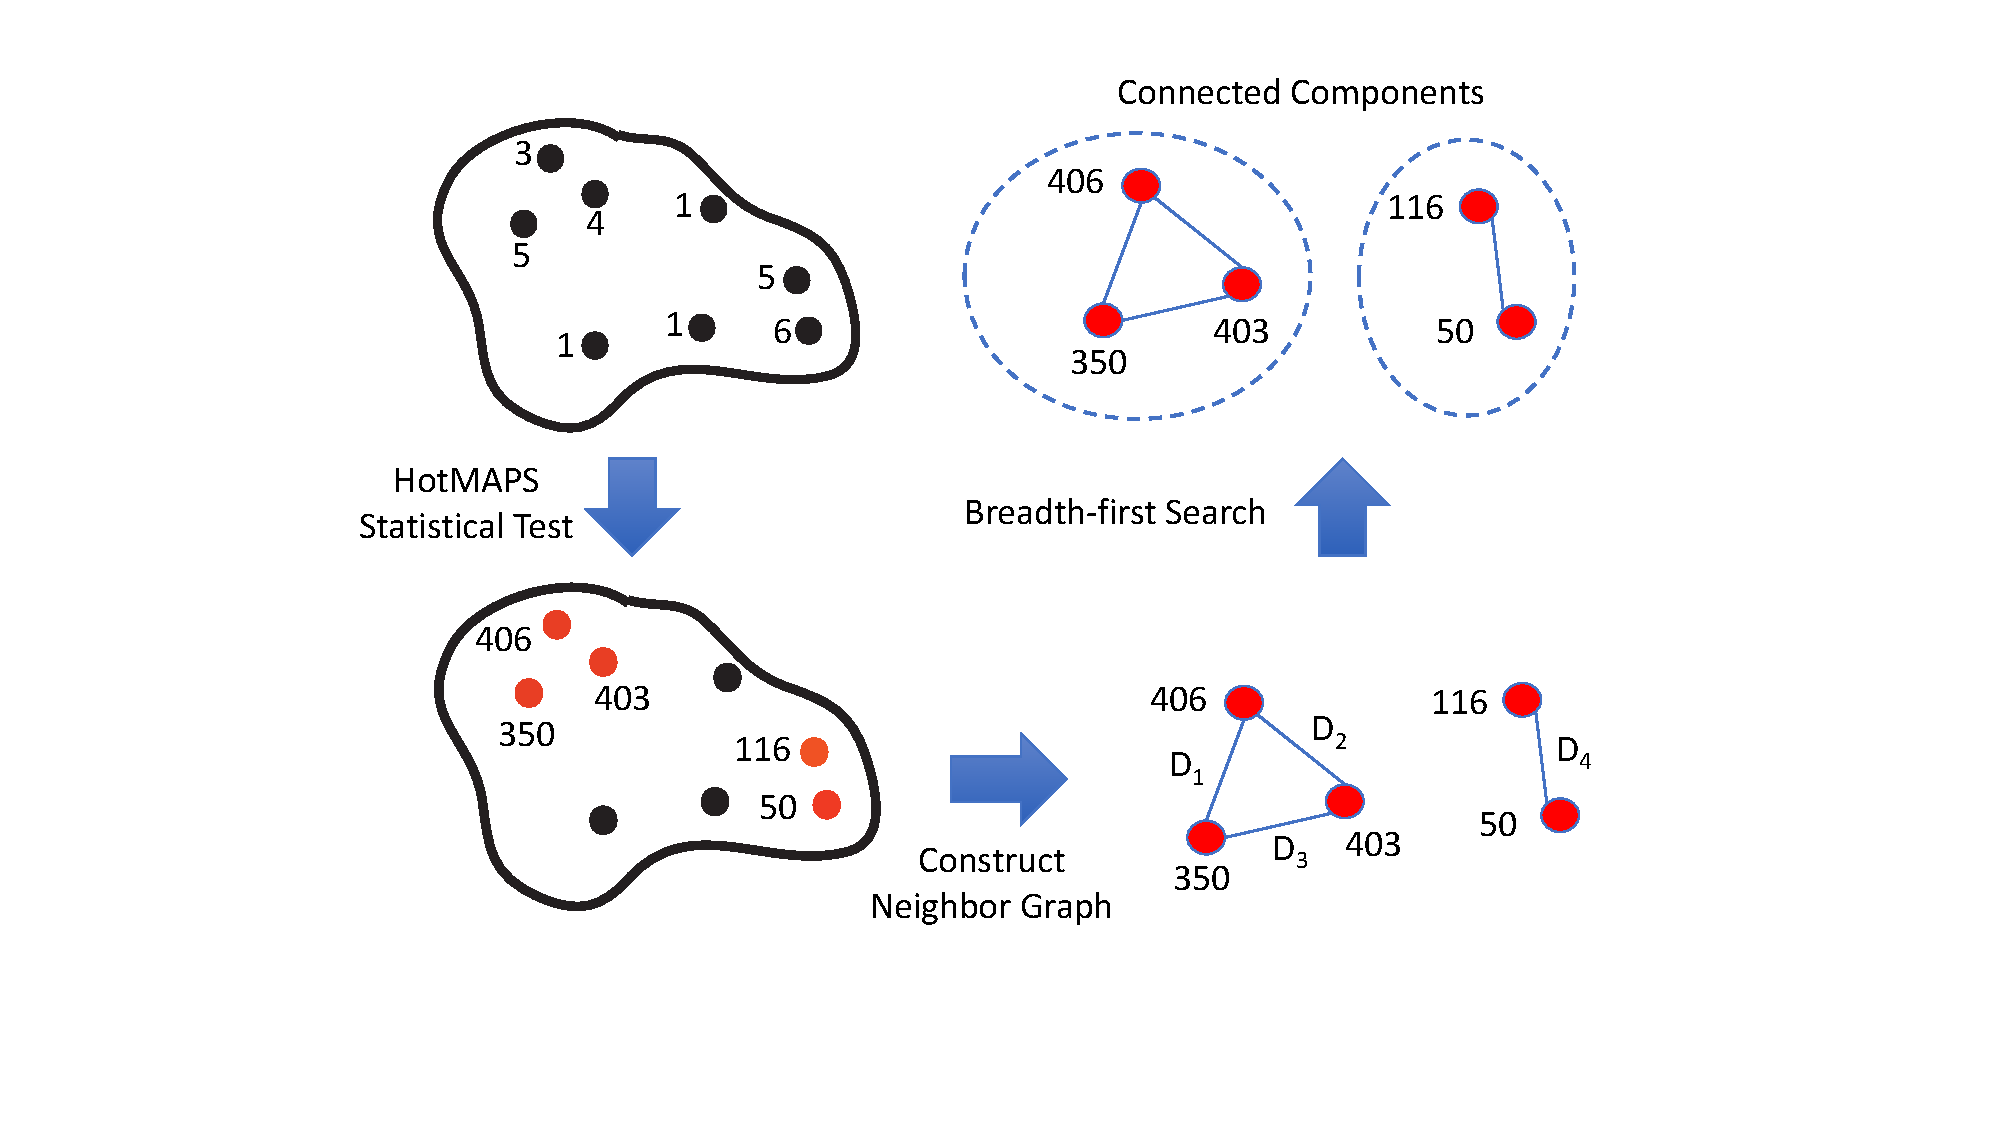
\includegraphics[width=0.9\linewidth]{figures/chapter5/hotmaps_algorithm.pdf}
  \caption[Algorithmic flowchart for Hotspot Missense mutation Areas in Protein Structure (HotMAPS) algorithm.]{HotMAPS was run on 65,372 protein structures and models.  For each structure or model, mutations were mapped from TCGA genomic coordinates to 3D protein space and for each mutated residue, its observed local mutation density was calculated. P-values were estimated based on simulations. If p-values for the same residue differed across multiple structures/models, the minimum was used and adjusted for multiple hypotheses testing with the Benjamini-Hochberg algorithm.  Hotspot regions were identified as connected components in a graph of significantly mutated residues.}
  \label{fig:hotmaps_algorithm}
\end{figure}

\subsection{Mutation density}

HotMAPS depends on calculating a mutation density for each amino acid residue. Let K be the set of all protein structures.  Each protein structure or model was an element $k\in K$.  For each k, the center of geometry in Euclidean space (i.e., centroid) was calculated for each residue ($r$), considering all backbone and side-chain atoms,

\begin{equation}
C_r^k = \frac{1}{|r|}\sum_{a\in r}{a}
\end{equation}

where $C_r^k$ is the center of geometry for residue $r$ in $k$, and a is a 3D position vector for each atom in residue $r$. The neighbors of residue $r$ were identified using a 10 angstrom radius cutoff from the center of geometry,

\begin{equation}
N_r^k = \{r' : dist(C_r^k, C_{r'}^k) \leq 10, r' \in R^k \}
\end{equation}

where $R^k$ is the set of residues for $k$, $N_r^k$ is the set of neighbor residues for residue $r$, and $dist$ is the Euclidean distance function. The density D of mutations at residue $r$ was calculated as the sum of mutations in the residue's neighborhood,

\begin{equation}
D_r^k = \sum_{n \in N_r^k}{M^k_n}
\end{equation}
\begin{equation}
D^k_{obs} = \{D^k_r : M^k_r>0, r \in R^k\}
\end{equation}

where $M_n^k$ is the number of missense mutations for the n'th residue neighbor, $D_r^k$ is the density of mutations for a specific residue and $k$, and $D_{obs}^k$ is the set of observed mutation densities for all mutated residues in a given $k$.

\subsection{Statistical model}

Next, I simulated the expected null hypothesis if mutations on the protein structure were under no selective pressure to occur in any particular region.   The null distribution is reasonably modeled by a discrete uniform distribution. Mutations occurring under the null were simulated by sampling with replacement a number of residues equal to the total observed mutations,

\begin{equation}
M_{sim}^k \sim Uniform(R^k, Size=\sum{M_r^k})
\end{equation}

where $M_{sim}^k$ is the simulated missense counts for all residues in $k$.  The procedure was modified slightly for protein complexes, which contain multiple protein chains that originate from a single gene product (e.g., a homodimer). I accounted for this non-independence by running identical simulations simultaneously on multiple duplicated protein chains.  Duplicate chains were identified based on either having same PDB chain letter and/or the same chain description. The mutation density for simulated mutations was calculated in the same manner as the observed mutations. The procedure was repeated for 10,000 iterations on each structure.

Based on the empirical null distribution established from simulations, I calculated the one-tailed p-value for each residue's mutation density being equal or larger,

\begin{equation}
P^k_r = \frac{\#\{d : d \geq D^k_r, d \in D^k_{sim}\}}{\#\{d \in D^k_{sim}\}}
\end{equation}

where $D_{sim}^k$ is the set of all simulated mutation densities and $P_r^k$ is the p-value for residue $r$ in $k$. Since there may be many structures and/or models that cover the same corresponding portion of the genome, multiple p-values were collapsed by taking the minimum p-value among residues that mapped to the same genomic codon. These unique genomic-level p-values were then corrected for multiple hypotheses by the Benjamini-Hochberg method \cite{RN94} and deemed significant at a q-value of 0.01. I selected the very conservative q=0.01 empirically, to minimize the number of false discoveries in our study.  Identifying the corresponding significant residues at the structure (or model) level was backtracked by using the supremum of significant p-values at the codon level as a cutoff,

\begin{equation}
P^* = \sup{\{P_c : q_c < 0.01, \forall c\}}
\end{equation}
\begin{equation}
R^k_{signif} = \{r : P^k_r \leq P^*, \forall r\}
\end{equation}

where $P_c$ and $q_c$ are the genomic p-value and q-value, respectively, for codon $c$, $P^*$ is the p-value cutoff adjusted for multiple hypotheses, $R_{signif}^k$ is the set of significant residues for $k$.

\subsection{Constructing hotspot regions}

3D mutation hotspot regions were identified as groupings of significant residues, according to the principle of maximum parsimony.  Specifically, I found the minimum number of non-contiguous hotspot regions that explained all significant residues. I first constructed a neighbor graph amongst significant residue positions, where edges were created if two residues could be considered as neighbors, defined as within 10 angstroms (1nm), which is the order of magnitude for the length of an amino acid residue side chain. 3D mutation hotspot regions for each k were then found as the connected components of the neighbor graph using breadth-first search. Our results were not very sensitive to small perturbations of this parameter (8\AA, 9\AA, 11\AA, 12\AA). The 10\AA maximum distance identified 85\% of the hotspot residues identified at the four other threshold values.

\section{Mapping mutations to protein structure}

\subsection{Mutational data set}

Mutation annotation format (MAF) file data for 23 tumor types from The Cancer Genome Atlas (TCGA) was downloaded by the Xena data store (\url{https://genome-cancer.soe.ucsc.edu/proj/site/xena/hub/}) using their API.

\subsection{Protein structure}

PDB structures were obtained from the Worldwide Protein Data Bank (PDB) (10/17/2015). Only structures solved by x-ray crystallography and containing at least one human protein chain were used.  To avoid computation on crystal-packing artifacts that are common in PDB multi-domain protein structures and proteins in complex with other proteins or DNA/RNA structures, I used PDB biological assemblies that model how proteins exist in vivo (\url{ftp://ftp.wwpdb.org/pub/pdb/data/biounit}). Additionally, single-domain, theoretical protein structure models constructed based on homology to non-human proteins were included to increase coverage over a greater proportion of genes. Theoretical models were obtained from the ModPipe human 2013 dataset (\url{ftp://salilab.org/databases/modbase/projects/genomes/H_sapiens/2013/}), built with Modeller 9.11 \cite{RN119}.   In addition to criteria required by ModPipe (ModPipe Protein Quality Score $>$ 1.1), theoretical models were further filtered to increase the quality of structures used in our assessment, requiring that: 1) models had a minimum length of 75 residues. 2) The sequence of the target human protein and the sequence of the non-human homolog used for homology modeling were $\geq$10\% identical. 3) The \q{loop} content of the protein model was $\leq$30\%. 4) Compactness score $C$ (see \autoref{eq:compactness}) was $\leq$1\AA/residue. The compactness score was based on the protein radius of gyration ($R_g$), and was employed to reject overly extended or unfolded structures. All thresholds were selected by visual inspection of structures meeting each of the four criteria.

Theoretical protein structure compactness score filter:
\begin{equation}
\label{eq:compactness}
C = \frac{4R_g}{N}
\end{equation}
\begin{equation}
\text{where } R_g=\sqrt{\frac{\sum_i{m_i(\vec{r}_i-\vec{r}_c)^2}}{\sum_i{m_i}}} 
\end{equation}

where N is total number of residues. $m_i$ is the mass of the i'th atom, $\vec{r}_i$ is the center of the i'th atom, and $\vec{r}_c$ is the protein center of geometry.

\subsection{Mapping algorithm}

Mapping of genome coordinates was done using a modified version of the TransMap algorithm (\autoref{fig:mapping_algorithm}), previously described in \cite{RN120}. In a minority of cases mutations did not have a one-to-one mapping within a protein structure (0.6\% of mutations analyzed in this study were impacted). Any hotspot region residue positions with ambiguous mappings were dropped from the final analysis. Protein sequences in the UniProt database (SwissProt curated only) \cite{RN121} were aligned to all transcripts in RefSeq, CCDS and Ensembl databases with tBLASTn \cite{RN122}.  Transcripts were then aligned to human genome assembly GRCh37 (hg19) with BLAT \cite{RN123}.  BLAT was also used to align the UniProt protein sequences with PDB SEQRES amino acid residue sequences (\autoref{fig:mapping_algorithm}).  For theoretical models, ModPipe provided a RefSeq or Ensembl transcript identifier and translation of each transcript into protein sequence, eliminating the need for the tBLASTn step to align protein sequence to transcript. 

\begin{figure}
  \centering
  \makeatletter
  \let\@currsize\normalsize
  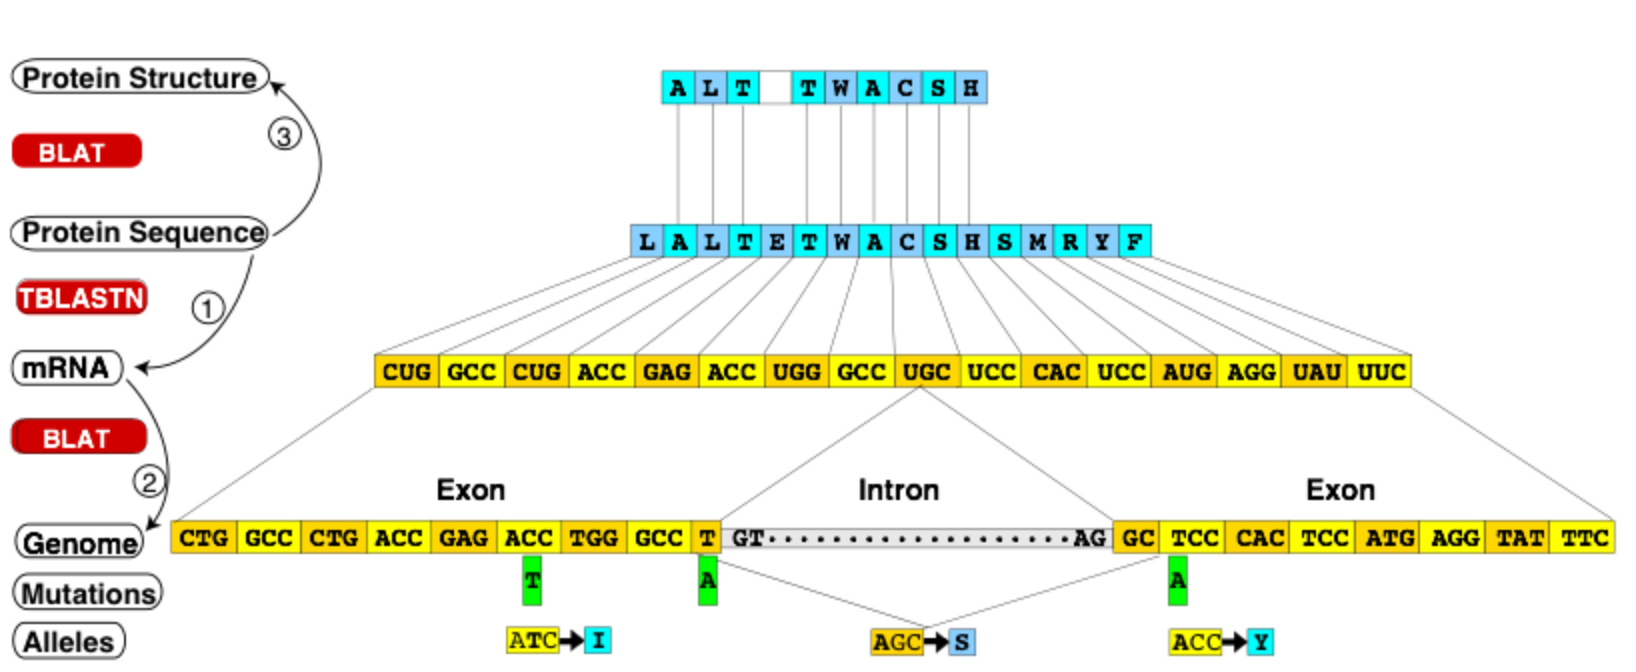
\includegraphics[width=0.9\linewidth]{figures/chapter5/mapping_algorithm.png}
  \caption[Mapping of genomic coordinates onto protein structures and models with a modified version of the TransMap algorithm.]{The mapping is done with three pairwise alignment steps, using tBLASTn and BLAT.  Projection of protein sequence coordinates to mRNA transcript coordinates (1) and finally genomic coordinates (2) is done \q{top down}. The process enables handling of split codons, such as the \q{AGC} shown.  Protein sequence coordinates are subsequently projected into the PDB coordinate system of protein structure (3).}
  \label{fig:mapping_algorithm}
\end{figure}

\section{3D mutation hotspot regions are important in cancer}

\subsection{3D hotspot regions are enriched in well-known cancer genes}

Among the set of genes with available protein structure or models (n = 15,697), the genes harboring a 3D hotspot region are enriched for OGs and TSGs (P = 6.1E−30 for OGs and P = 2.4E−13 for TSGs; one-tailed Fisher exact test). They are also enriched for genes in the CGC list (P = 1.4E−30; one-tailed Fisher exact test). The subset of these genes harboring only a 3D hotspot region not detectable in 1D is also significantly enriched (P = 4.3E−09 for OGs, P = 7.9E−12 for TSGs, P = 8.0E−11 for CGC genes; one-tailed Fisher exact test). An additional 23 genes that are proposed OGs, TSGs, and/or drug targets or hereditary cancer genes contained at least one 3D hotspot region. This enrichment of known and candidate driver genes supports my claim that many of the regions are biologically relevant and not simply artifacts. While regions were detected in only approximately 18\% of established cancer genes, I expect that many of these genes harbor drivers other than missense mutations, some are drivers in tumor types not represented in our study and many lack structural coverage.

\subsection{Mutations in 3D hotspot regions are different from other somatic mutations in cancers}

I examined whether the amino acid residue positions and the missense mutations in the 3D hotspot regions had distinctive features suggestive of a special biologic importance, when compared with the remaining mutations in our study. Four candidate distinguishing features were tested: (i) vertebrate evolutionary conservation; (ii) occurrence at a protein-protein interface, which increases the potential for a missense mutation to disrupt protein-protein interactions; (iii) \textit{in silico} cancer driver scores generated with the CHASM algorithm \cite{RN29}; and (iv) in silico pathogenicity scores generated with the VEST algorithm \cite{RN30}, which are predictors of increased missense mutation impact (\autoref{fig:hotspot_properties}). In comparison with mutated residues not in 3D hotspot regions, vertebrate evolutionary conservation was higher and protein-protein interface occurrence was higher in the 3D hotspot regions (conservation P = 2.9E−29, Mann-Whitney U test; protein interface P = 5.2E−13, one-tailed Fisher exact test). In silico driver scores and pathogenicity scores were higher for missense mutations in 3D hotspot regions (driver score P = 3.0E−47, pathogenicity score P = 3.0E−16; Mann-Whitney U-test) than for the remaining mutations (\autoref{fig:hotspot_properties}).

\begin{figure}
  \centering
  \makeatletter
  \let\@currsize\normalsize
  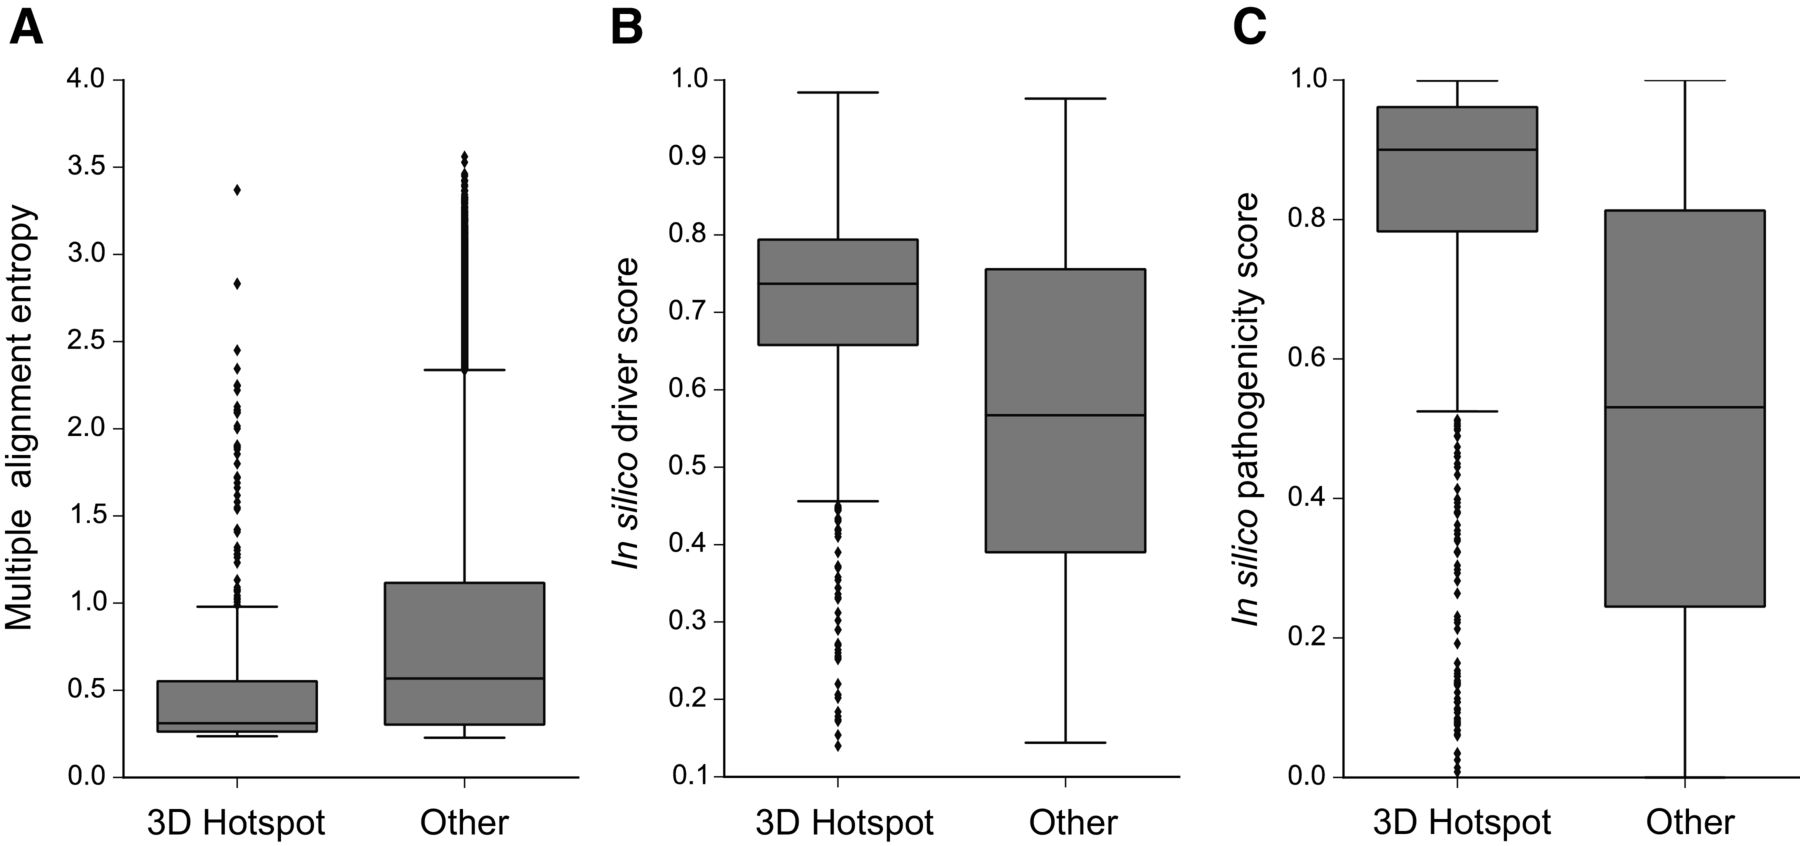
\includegraphics[width=0.9\linewidth]{figures/chapter5/hotspot_properties.jpg}
  \caption[3D hotspot regions are different from other mutated protein residues.]{Three distinguishing features of HotMAPS regions. A, HotMAPS-mutated residues are more conserved in vertebrate evolution than mutated residues not in hotspot regions, as shown by lower multiple alignment entropy (P = 1.2E−29; Mann-Whitney U test). Multiple alignment entropy is calculated as the Shannon entropy of protein-translated 46-way vertebrate genome alignments from UCSC Genome Browser, which is lowest for the most conserved residues. B and C, HotMAPS missense mutations have higher in silico cancer driver scores from the CHASM algorithm (P = 5.3E−47; Mann-Whitney U test) than those mutations not in hotspot regions (B) and higher in silico pathogenicity scores from the VEST algorithm (P = 7.0E−162; Mann-Whitney U test; C). Finally, HotMAPS-mutated residues occur more frequently at protein-protein interfaces (P = 1.3E−11; one-tailed Fisher exact test).}
  \label{fig:hotspot_properties}
\end{figure}

\subsection{3D hotspot regions are different in oncogenes and tumor suppressor genes}

The catalog contains 37 regions stratified by tumor type in bonafide tumor suppressor genes and 77 in bonafide oncogenes (114 regions in 30 genes), using as a benchmark the classifications of Vogelstein and colleagues (landscapes benchmark; \cite{RN25}). I used these data to explore possible differences between tumor suppressor gene and oncogene regions at amino acid resolution. I found that in tumor suppressor genes, 3D hotspot regions were larger than in oncogenes (region size P = 9.6E−06; Mann-Whitney U test). They were also more mutationally diverse (mutational diversity P = 2.1E−07; Mann-Whitney U test). In addition, oncogene 3D hotspot regions were more conserved in vertebrate evolution and more solvent accessible in protein structure, meaning that they tend to occur at the protein surface (evolution P = 4.7E−07, solvent accessible P = 1.5E−06; Mann-Whitney U test). Hotspot regions in tumor suppressor genes harbored increased net change in hydrophobicity (P = 3.3E−07; Mann-Whitney U test) and net change in volume (P = 2.2E−07; Mann-Whitney U test), suggesting that their impact on protein function could be due to decreased stability. The in silico missense mutation cancer driver scores were higher for oncogene regions (P = 0.003; Mann-Whitney U test). I also tested differences between in silico pathogenicity scores and occurrence at protein-protein interfaces between OG and TSG regions, but these were not significant (pathogenicity scores P = 0.37, protein interface P = 0.34; Mann-Whitney U test).

The fact that these differences between oncogene and tumor suppressor gene regions were statistically significant suggested that they might have predictive value. Principal components analysis (PCA) of the six significant features indicated some separation (\autoref{fig:hotmaps_pca}A). Next, I trained a Naive Bayes machine learning classifier to discriminate between oncogene and tumor suppressor gene hotspot regions, using region size, mutational diversity, vertebrate conservation, residue solvent accessibility, mutation net hydrophobicity change, and residue volume change as features. A rigorous gene-level holdout protocol was used to avoid overfitting. A Naive Bayes score closer to 1.0 indicates that the hotspot region is likely in an OG while a score closer to 0.0 indicates that it is in a TSG. Area under receiver operating characteristic (ROC) curve or AUC, a standard measure of classifier performance, was 0.84 out of 1.0, a result that supports my claim that 3D hotspot regions in oncogenes and tumor suppressor genes have distinctive characteristics (\autoref{fig:hotmaps_pca}B). AUC of a classifier with random performance is 0.5. Performance did not improve when the other features were included in the classifier. The ROC performance and PCA plot support my claim that characteristic differences between oncogenes and tumor suppressor genes hotspots can be quantified. 

\begin{figure}
  \centering
  \makeatletter
  \let\@currsize\normalsize
  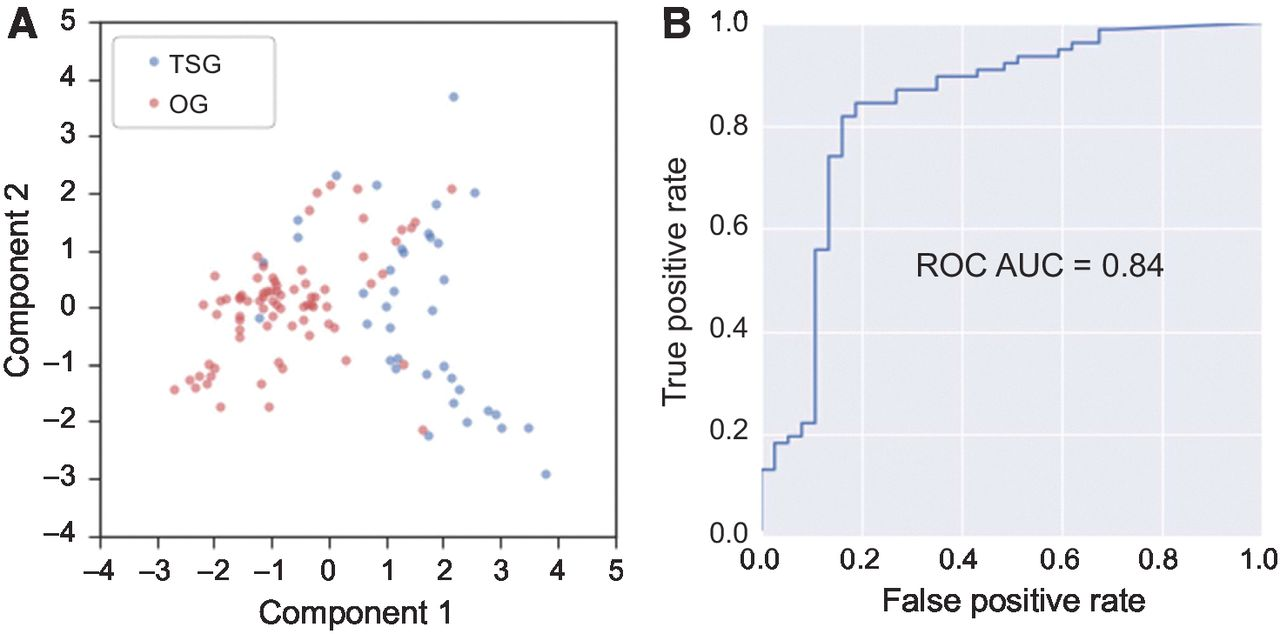
\includegraphics[width=0.9\linewidth]{figures/chapter5/pca.jpg}
  \caption[HotMAPS regions have different characteristic features in OGs and TSGs.]{A, PCA plot shows a clustering pattern in hotspot regions identified in oncogenes (OG=red) and tumor suppressor genes (TSG=blue). Each point is a region represented by six numeric features, projected into two dimensions. The features are region size, mutational diversity, vertebrate evolutionary conservation, residue relative solvent accessibility, mutation net change in hydrophobicity, and mutation net change in residue volume. B, OG and TSG HotMAPS regions can be discriminated with machine learning, based on six features. A Gaussian Naive Bayes classifier trained with the landscapes benchmark provides a reasonable separation between the two classes with AUC = 0.84 out of 1.0. Performance of a random classifier is AUC = 0.5. ROC, receiver operating characteristic; AUC, area under the ROC curve.}
  \label{fig:hotmaps_pca}
\end{figure}

\subsection{What is gained by 3D hotspot region detection versus 1D?}

The larger size and mutational diversity of hotspot regions in tumor suppressor genes (TSGs) versus oncogenes (OGs) suggest that they could be more difficult to detect and perhaps they have been underreported by 1D approaches. OG hotspot regions consisting of recurrent missense mutations at one or two residues can be seen by eye with lollipop plots and are straightforward to detect computationally based on 1D primary sequence. I hypothesized that detection of many TSG hotspot regions might require a 3D algorithm. To maximize the interpretability of this analysis, regions that occurred in multiple tumor types were merged so that each region was represented only once in each gene.

For a well-controlled comparison of 3D and 1D hotspot region detection, I applied a 1D version of our method to the protein chain sequences of the same set of PDB protein bioassemblies and theoretical protein structure models to detect nonuniform clustering patterns on primary protein sequence. Seventy-two percent of hotspot regions identified in 3D were identifiable in 1D.

Next, I compared the number of hotspot regions identified in OGs and TSGs. I considered regions identified in 3D only, in both 3D and 1D, and in 1D only. Using the bona fide OGs and TSGs (\autoref{tab:hotmaps_main}), there were significantly more OG regions that TSG regions identified by the 1D algorithm (P = 0.03; one-sided Fisher exact test). The 1D-only version of the algorithm detected 5 OG and 2 TSG regions; 1D further detected an additional 25 OG and 7 TSG regions that were also identified by the 3D algorithm. The 3D algorithm identified an additional 4 OG and 6 TSG regions. To increase our power, I repeated this test again using the bona fide OGs and TSGs plus additional regions in five candidate OGs and TSGs reported in the literature (OGs were FSIP2, MTOR, RANBP2, CHEK2, and MAPK1; TSGs were RASA1, SMARCA2, KEAP1, CUL1, TGFBR2; all are listed and cited in \autoref{tab:hotmaps_second}), yielding increased statistical significance (P = 0.009, one-sided Fisher exact test). The results suggest that 1D detection methods may be better suited to detecting regions in OGs rather than TSGs.

\begin{table}
  \centering
  \makeatletter
  \let\@currsize\normalsize
  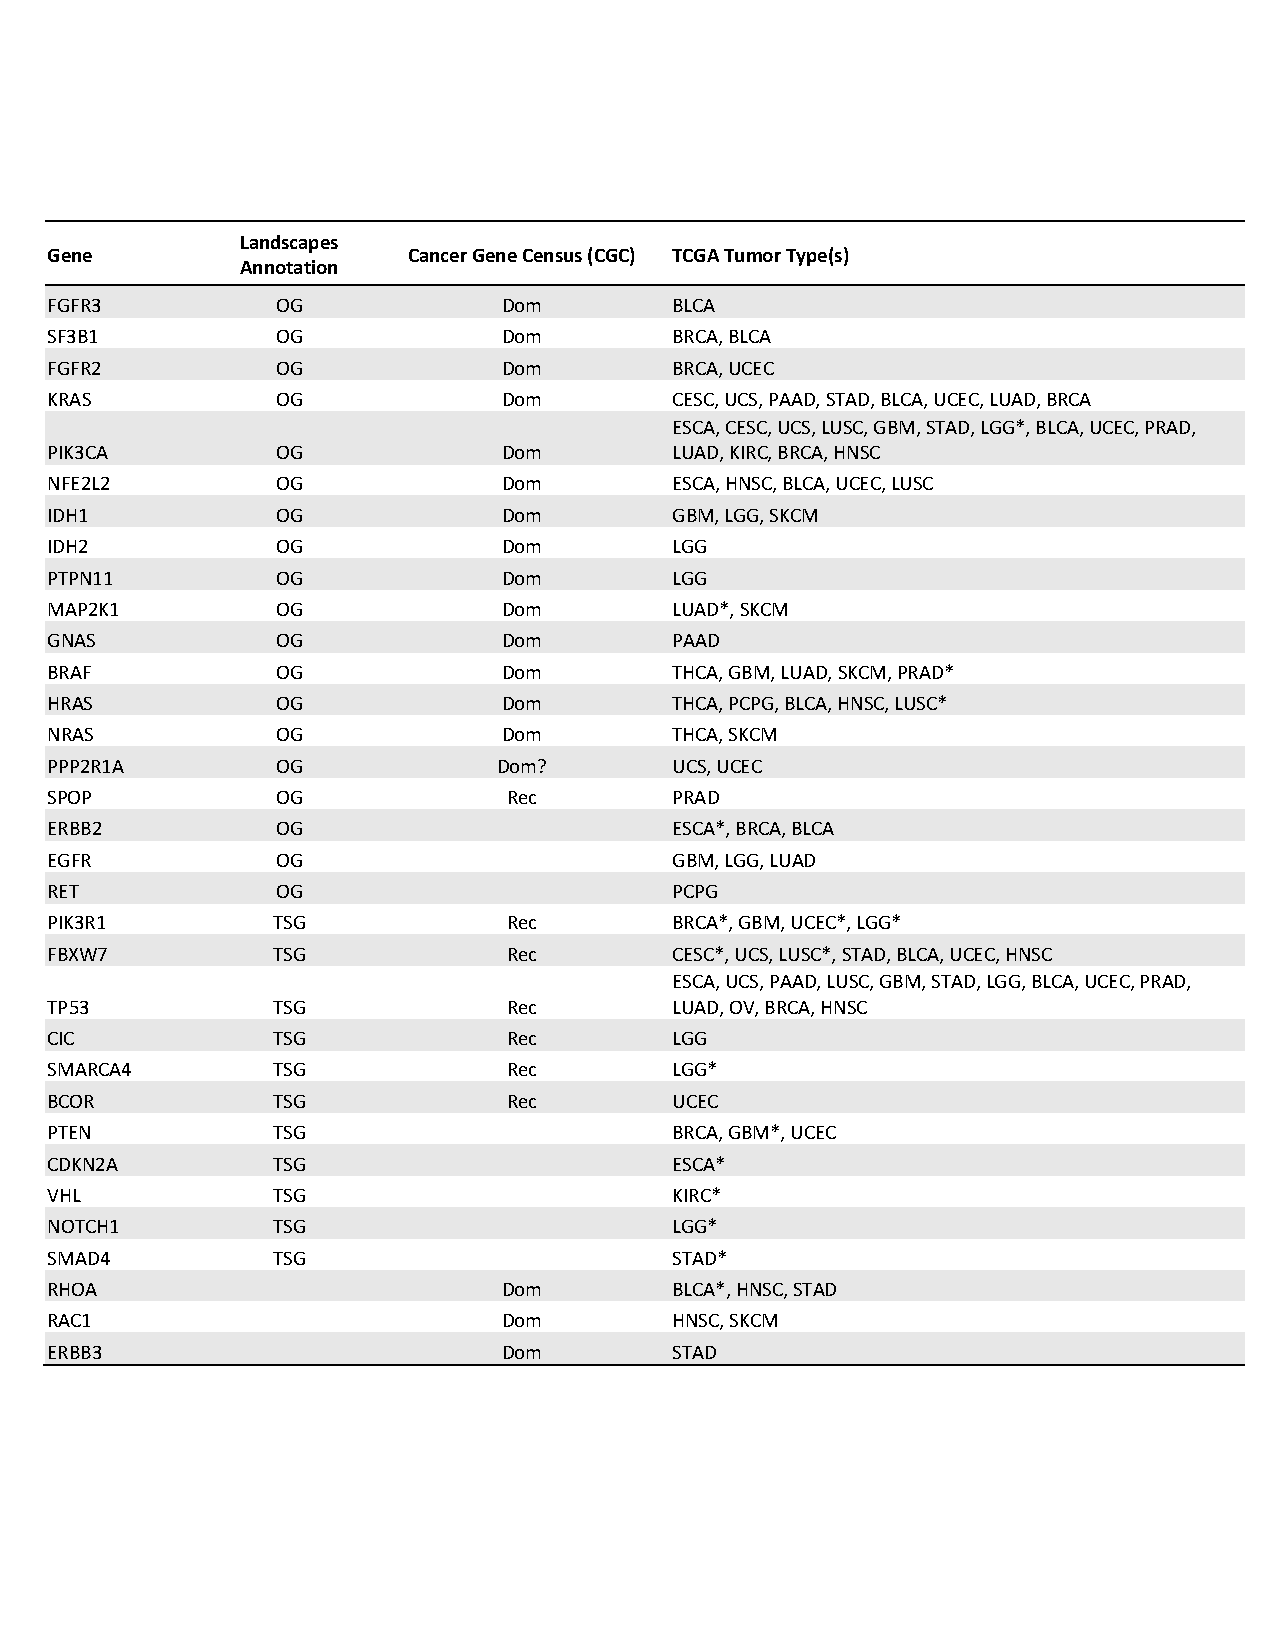
\includegraphics[width=\linewidth]{tables/chapter5/HotMAPS_main_table.pdf}
  \caption[3D HotMAPS regions in known cancer genes]{Cancer genes with 3D HotMAPS regions identified in TCGA tumor types and in landscapes benchmark or cancer gene census}
  \label{tab:hotmaps_main}
\end{table}

\begin{table}
  \centering
  \makeatletter
  \let\@currsize\normalsize
  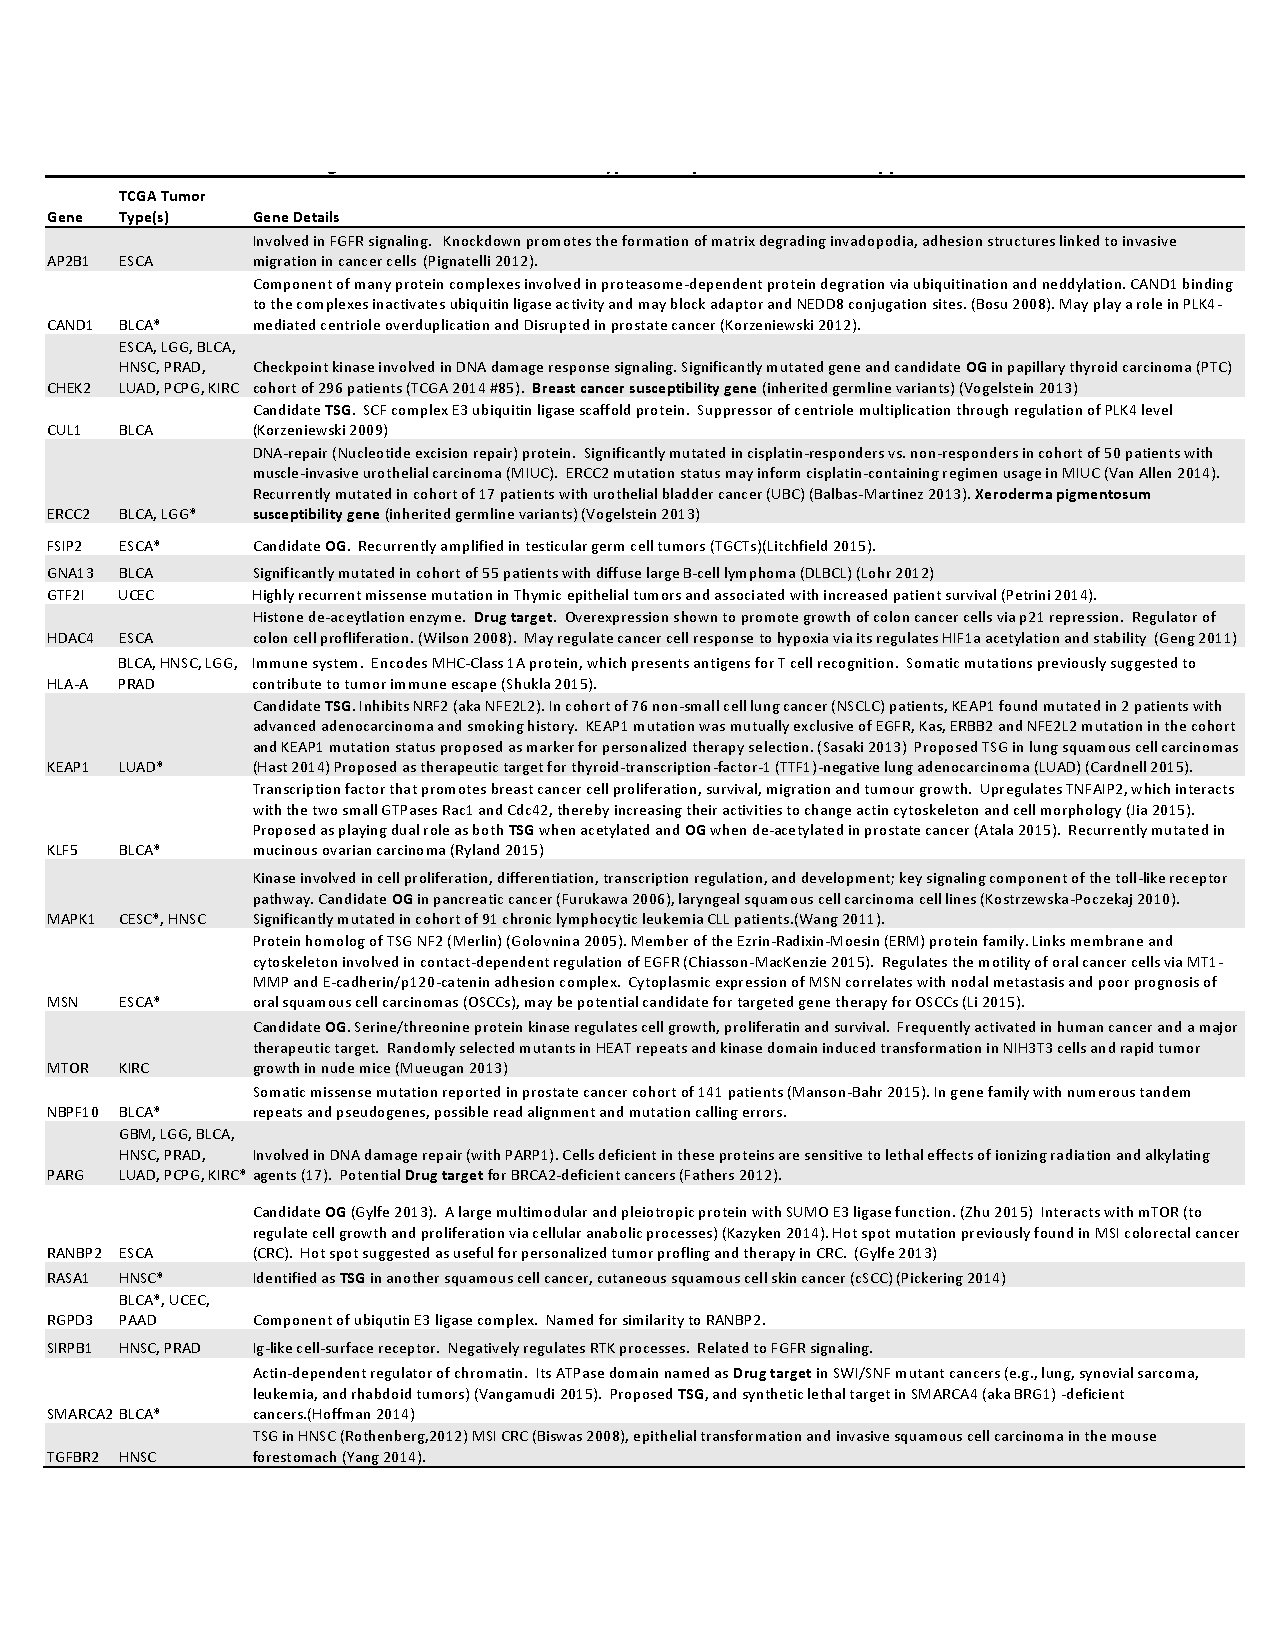
\includegraphics[width=\linewidth]{tables/chapter5/HotMAPS_second_table.pdf}
  \caption[3D HotMAPS regions with supportive evidence]{Genes with HotMAPS regions identified in TCGA tumor types}
  \label{tab:hotmaps_second}
\end{table}

A further problem with sequence-based 1D hotspot region detection is that larger regions detectable in 3D may be only partially characterized and/or split into multiple pieces. \autoref{fig:benefits_3d_space} shows an example of a TSG hotspot region in FBXW7 found in 3D by HotMAPS that has been split into two pieces by the 1D algorithm. In 1D protein sequence, residue 465 is not close enough to residues 502 and 505 to be identified in one hotspot region. On the 3D protein structure of FBXW7 (PDB code 2OVQ), the three residues are spatially close and a single hotspot region is detected.

\begin{figure}
  \centering
  \makeatletter
  \let\@currsize\normalsize
  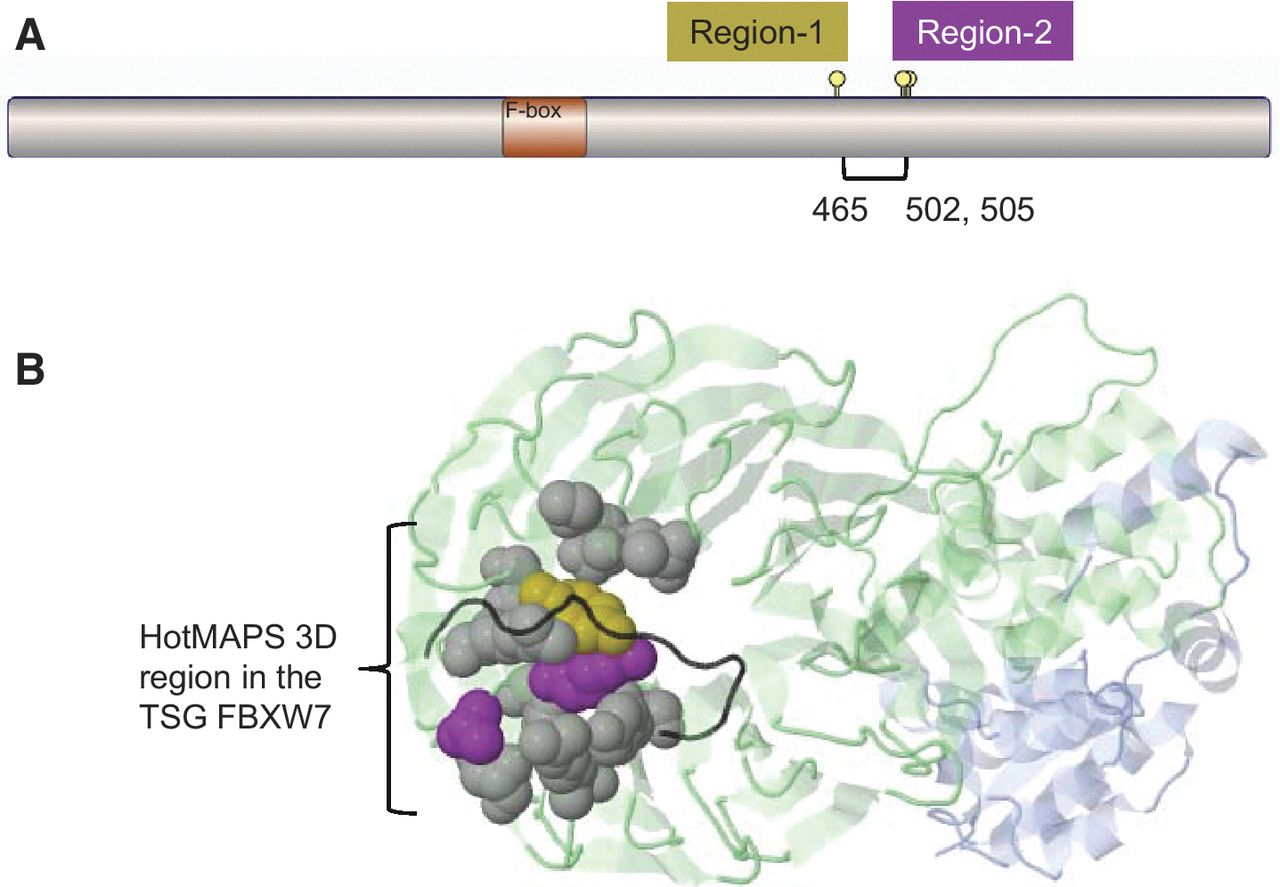
\includegraphics[width=0.9\linewidth]{figures/chapter5/benefits_3d_space.jpg}
  \caption[Comparison of hotspot detection in the TSG FBXW7 in 1D and 3D.]{Comparison of hotspot detection in the TSG FBXW7 in 1D and 3D. A, a simplified 1D version of HotMAPS found two regions in FBXW7. The 3D version of HotMAPS found a single larger region, encompassing both regions. Diagram shows protein sequence of FBXW7, which contains a single F-box functional domain. Region-1, residue 465 (left lollipop); Region-2, residues 502 and 505 (right lollipops). B, HotMAPS identifies a single 3D hotspot region in FBXW7. Structure of SCFFbw7 ubiquitin ligase complex (PDB 2OVQ), containing FBXW7 (green), SKP1 (blue), and CCNE1 fragment (degron peptide; black). Residue coloring: 1D Region-1, gold; 1D Region-2, purple. Residues missed by 1D detection but included in HotMAPS 3D, gray. Although the 1D regions are far in the primary protein sequence, residues 505 and 465 spatially contact at the interface with CCNE1. Protein structure figures were generated by JSMol in MuPIT (\url{http://mupit.icm.jhu.edu/}).}
  \label{fig:benefits_3d_space}
\end{figure}

\section{3D hotspot regions may increase interpretability of driver mechanisms}

Three-dimensional consideration of hotspot regions in protein structure can potentially provide researchers with a rich source of hypothesis generation about driver mechanisms. While gene- or domain-level mutation enrichment analysis can point to potential protein functions, interactions, biologic processes, and pathways important for cancer etiology and progression, more detailed information may be available once a specific set of mutated amino acid residues has been identified as significant.

For many of the 3D hotspot regions found by HotMAPS, the literature contains evidence that they are in direct contact with or proximal to amino acid residues of known functional importance. \autoref{fig:hotmaps_examples} shows six cancer-associated proteins in which the hotspot region is either overlapping or proximal to important functional sites.

\begin{figure}
  \centering
  \makeatletter
  \let\@currsize\normalsize
  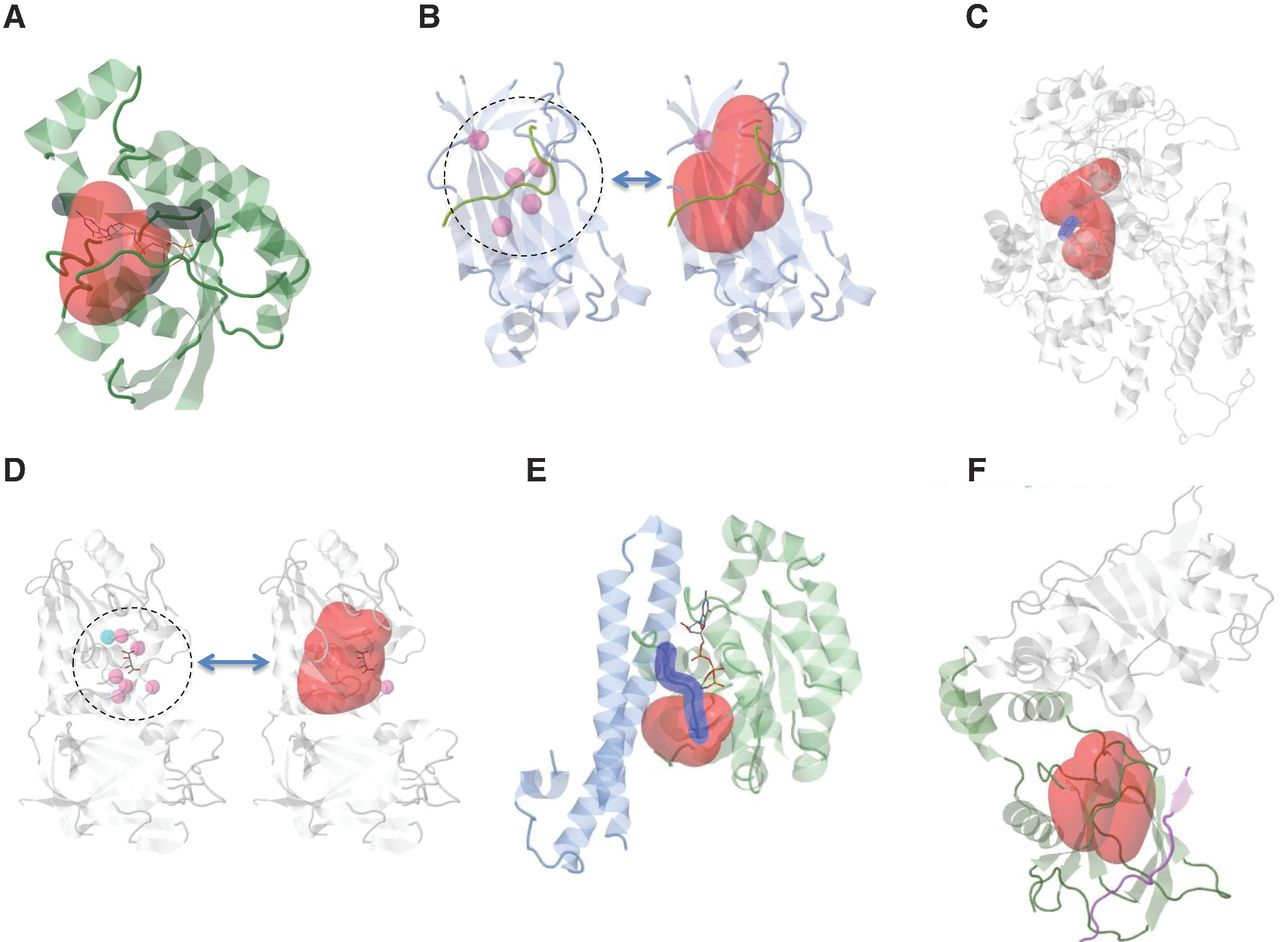
\includegraphics[width=0.9\linewidth]{figures/chapter5/hotmaps_examples.jpg}
  \caption[HotMAPS hotspot regions overlap and are proximal to important functional sites.]{HotMAPS hotspot regions overlap and are proximal to important functional sites. A, HNSCC hotspot region (red) in RAC1 (green) and GTP/GDP-binding residues (dark gray; PDB 2FJU). B, PRAD hotspot region (red) in SPOP-substrate complex (PDB 3HGH) with SPOP (blue) and H2AFY substrate (green). Left, five residues (pink) that when mutated show strongly reduced affinity for substrate. C, BLCA hotspot region (red) in ERCC2 (gray) shown on theoretical model of ERCC2 helicase ATP-binding domain. The hotspot is proximal to the DEAH box (blue), a highly conserved motif containing residues that interact with Mg2+ and are critical for ATP-binding and helicase activity. D, UCEC hotspot region (red) in PTEN (PDB 1D5R) with active site phosphocysteine residue (blue), residues when mutated annotated to reduce phosphatase activity (pink). E, STAD hotspot region (red) in RHOA with a GTP analog bound (sticks; PDB 1CXZ). GTP-binding residues and effector region, dark blue. F, KIRC hotspot region (red) in VHL-TCEB1-TCEB2 complex, bound to HIF1A peptide (PDB 4AJY). Proximity to the interaction site of VHL (green) and HIF1A (blue) suggests possible decreased ubiquitination of HIF1A, resulting in increased protein expression of HIF1A. TCEB1 and TCEB2, gray.}
  \label{fig:hotmaps_examples}
\end{figure}

\subsection{RAC1 hotspot in squamous head and neck cancer}
RAC1 is a Rho GTPase important in signaling systems that regulate the organization of actin cytoskeleton and cell motility. The hotspot overlaps the GTP/GDP-binding site and could impact regulation of normal RAC1 cycling between GTP- and GDP-bound states (\autoref{fig:hotmaps_examples}A). It contains a previously identified recurrent mutation in melanoma (P29S), which dysregulates RAC1 by a fast cycling mechanism \cite{RN124}.

\subsection{SPOP hotspot in prostate cancer (PRAD)}
SPOP is the substrate recognition component of a cullin3-based E3 ubiquitin-protein ligase complex, which targets multiple substrates for proteasomal degradation. The hotspot overlaps with a binding groove harboring five residue positions (pink) where mutagenesis has strongly reduced affinity for the substrate (annotated in the UniProtKB) (\autoref{fig:hotmaps_examples}B).

\subsection{ERCC2 hotspot in bladder cancer}
ERCC2 is an ATP-dependent helicase that is part of the protein complex TFIIH involved in RNA polymerase II transcription and nucleotide excision repair (NER). I identified a hotspot region, proximal to the DEAH box, a highly conserved motif containing residues that interact with Mg2+ and are critical for ATP binding and helicase activity (\autoref{fig:hotmaps_examples}C). This proximity suggests that the hotspot mutations could disrupt ATPase activity and yield defective NER \cite{RN125}.

\subsection{PTEN hotspot}
PTEN is a phosphatase for both proteins and phosphoinositides, and it removes a phosphate from PIP3, critical for signaling to AKT. The hotspot region identified in endometrial cancer (UCEC) spans two functionally important loops in the protein (P and WPD loops) at the boundary of the active site pocket (\autoref{fig:hotmaps_examples}D). Residues in these loops are critical for catalysis (blue dot) and are important for the P-loop's conformation. Mutagenesis of residues in the WPD loop reduces phosphatase activity and increases colony formation in cell culture \cite{RN126}. Pink dots show residues that impact phosphatase activity.

\subsection{RHOA hotspots}
RHOA is a small GTPase oncogene, and like RAC1 is a member of the Ras superfamily \cite{RN127}. I identified hotspot regions in bladder cancer (BLCA), head and neck squamous cell cancer (HNSCC), and stomach adenocarcinoma (STAD). The hotspot regions overlap with the RHOA effector region, a highly conserved motif that is involved in Ras superfamily signaling with downstream effector proteins (\autoref{fig:hotmaps_examples}E). The regions are immediately proximal to a magnesium ion, which has been implicated in regulating the kinetics of Rho family GTPases \cite{RN128}.

\subsection{VHL hotspot (KIRC)}
VHL is a component of an E3 ubiquitin protein ligase complex, and it ubiquitinates the OG transcription factor HIF1A, targeting it for proteasomal degradation \cite{RN129}. One impact of VHL loss of function with failure to ubiquitinate HIF1A is increased protein expression of HIF1A. The hotspot region is proximal to its interaction site with HIF1A and could potentially have an impact on this interaction (\autoref{fig:hotmaps_examples}F). The TCGA kidney cancer (KIRC) samples were stratified on the basis of their missense mutation status: VHL hotspot, non-hotspot, or no missense (WT). HIF1A protein expression was not significantly different between VHL non-hotspot and VHL WT groups (P = 0.5; Mann-Whitney U test), but was significantly higher between VHL hotspot and VHL WT groups (P = 0.03; Mann-Whitney U test). This result is consistent with a special role for VHL hotspot missense mutations in regulating HIF1A protein expression. However, increased HIF1A expression in these KIRC samples is likely impacted by additional genetic and other factors. I might see a substantially lower P value if VHL hotspot mutations were the only cause of the observed increase. Also, there are many VHL missense mutations outside of the hotspot region, and it is likely that several of these also have a functional impact. In particular, several of them are at the interface of VHL and the TCEB1 and TCEB2 in the complex and could impact VHL/TCEB binding.

\section{Conclusions}

I systematically identified 3D missense hotspot regions using TCGA somatic mutation data from 6,594 samples in 23 tumor types. HotMAPS identified 107 unique regions and 216 cancer type-specific regions. This catalog enables assessment of how the specific missense mutations in a hotspot contribute to cancer-associated molecular mechanisms. Unlike many machine learning algorithms, the visualization of HotMAPS region with protein structure allows model interpretability by biologists with domain knowledge of a particular protein.

At the time of publication, several other algorithms were published which also supported the notion that mutational clustering in protein structure was advantageous \cite{RN133, RN131, RN132}. In a comparison from \cite{RN133}, HotMAPS had performance equivalent to other top methods on discriminating likely driver missense mutations from an \textit{in vivo} experiment. The HotMAPS algorithm does have similarities with the DBSCAN algorithm \cite{RN117}, which is also based on using density estimates for clustering. However, DBSCAN does not have a statistically principled criterion for controlling false discoveries. 

Although recurrent missense mutations have long been known to occur in both oncogenes and tumor suppressor genes \cite{RN107}, they have been observed more frequently in oncogenes. Here I showed that there are systematic differences in hotspot regions found in oncogenes and tumor suppressor genes. Oncogene regions are smaller, less mutationally diverse, more evolutionarily conserved, and more solvent accessible than tumor suppressor gene regions. Tumor suppressor gene regions are more likely to harbor mutations that may impact protein stability through changes in hydrophobicity or volume. Potential explanations for these differences are that there are more ways to lose the function of a protein than to gain function \cite{RN130}. Loss-of-function tumor suppressor mutations can occur at many residue positions and involve many types of amino acid residue substitutions, while oncogene mutations will occur at a few functionally important positions and involve fewer substitution types.

